\documentclass[a4paper]{article}
\usepackage[a4paper,margin=25mm]{geometry}
\usepackage{graphicx,subcaption}
\usepackage{amsmath,amsfonts}
\usepackage{qtree}
\usepackage{tikz}
\usetikzlibrary{arrows,arrows.meta,quotes}
\usepackage{varwidth}

\begin{document}

%%%%%%%%%%%%%%%%%%%%%%%%%%%%%%%%%%%%%%%%%%%%%
% HMM
\begin{figure}[hbt]
\centering
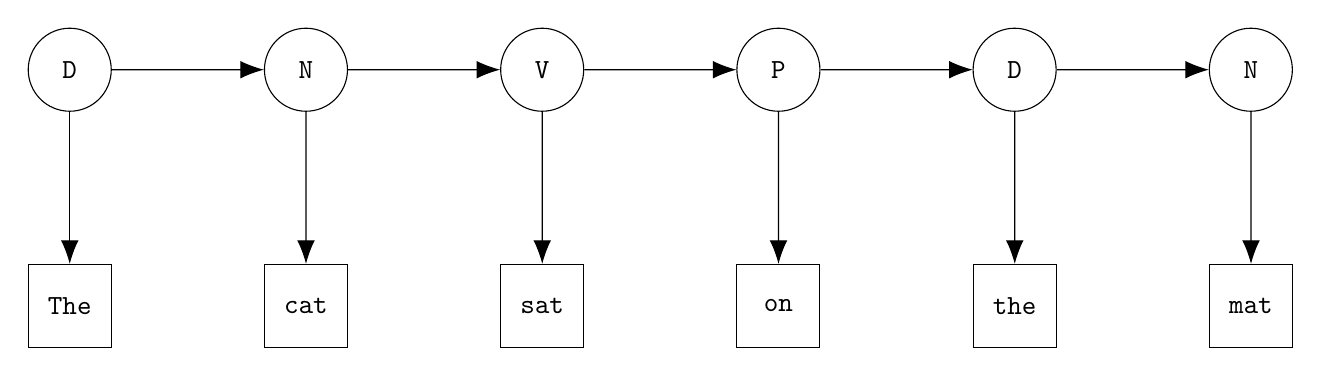
\begin{tikzpicture}[
  scale=1.5,
  cnode/.style={draw,circle,minimum size=3em,inner sep=3pt},
  snode/.style={draw,rectangle,minimum size=3em,inner sep=3pt}
]
  % tokens
  \node[snode] (y1) at (0,0) {$\texttt{The}$};
  \node[snode] (y2) at (2,0) {$\texttt{cat}$};
  \node[snode] (y3) at (4,0) {$\texttt{sat}$};
  \node[snode] (y4) at (6,0) {$\texttt{on}$};
  \node[snode] (y5) at (8,0) {$\texttt{the}$};
  \node[snode] (y6) at (10,0) {$\texttt{mat}$};

  % states
  \node[cnode] (s1) at (0, 2) {$\texttt{D}$};
  \node[cnode] (s2) at (2, 2) {$\texttt{N}$};
  \node[cnode] (s3) at (4, 2) {$\texttt{V}$};
  \node[cnode] (s4) at (6, 2) {$\texttt{P}$};
  \node[cnode] (s5) at (8, 2) {$\texttt{D}$};
  \node[cnode] (s6) at (10, 2) {$\texttt{N}$};

  % edges
  \draw[-{Latex[length=3mm]}] (s1) edge (y1);
  \draw[-{Latex[length=3mm]}] (s1) edge (s2);
  \draw[-{Latex[length=3mm]}] (s2) edge (y2);
  \draw[-{Latex[length=3mm]}] (s2) edge (s3);
  \draw[-{Latex[length=3mm]}] (s3) edge (y3);
  \draw[-{Latex[length=3mm]}] (s3) edge (s4);
  \draw[-{Latex[length=3mm]}] (s4) edge (y4);
  \draw[-{Latex[length=3mm]}] (s4) edge (s5);
  \draw[-{Latex[length=3mm]}] (s5) edge (y5);
  \draw[-{Latex[length=3mm]}] (s5) edge (s6);
  \draw[-{Latex[length=3mm]}] (s6) edge (y6);
\end{tikzpicture}
\end{figure}

%%%%%%%%%%%%%%%%%%%%%%%%%%%%%%%%%%%%%%%%%%%%%
% hierarchical derivation
\begin{figure}[hbt]
\centering
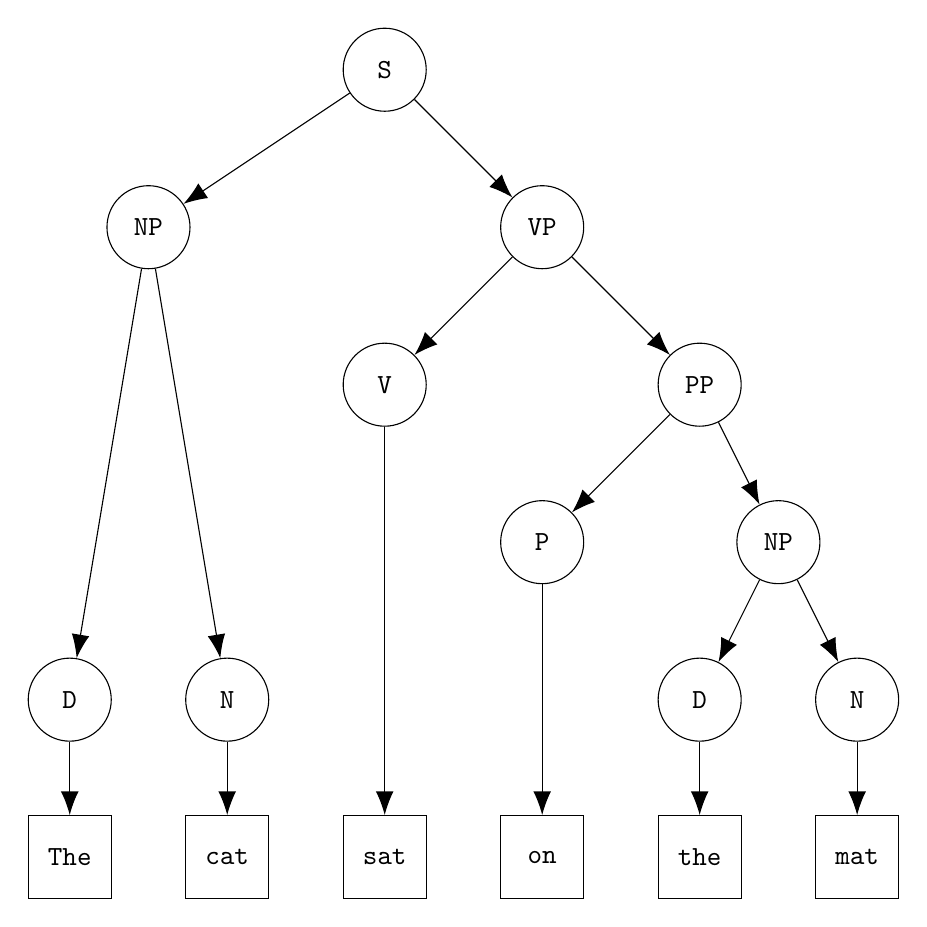
\begin{tikzpicture}[
  scale=1.0,
  cnode/.style={draw,circle,minimum size=3em,inner sep=3pt},
  snode/.style={draw,rectangle,minimum size=3em,inner sep=3pt}
]
  % tokens
  \node[snode] (y1) at (0,0) {$\texttt{The}$};
  \node[snode] (y2) at (2,0) {$\texttt{cat}$};
  \node[snode] (y3) at (4,0) {$\texttt{sat}$};
  \node[snode] (y4) at (6,0) {$\texttt{on}$};
  \node[snode] (y5) at (8,0) {$\texttt{the}$};
  \node[snode] (y6) at (10,0) {$\texttt{mat}$};

  % states
  \node[cnode] (s1) at (0, 2) {$\texttt{D}$};
  \node[cnode] (s2) at (2, 2) {$\texttt{N}$};
  \node[cnode] (s3) at (4, 6) {$\texttt{V}$};
  \node[cnode] (s4) at (6, 4) {$\texttt{P}$};
  \node[cnode] (s5) at (8, 2) {$\texttt{D}$};
  \node[cnode] (s6) at (10, 2) {$\texttt{N}$};

  % token edges
  \draw[-{Latex[length=3mm]}] (s1) edge (y1);
  \draw[-{Latex[length=3mm]}] (s2) edge (y2);
  \draw[-{Latex[length=3mm]}] (s3) edge (y3);
  \draw[-{Latex[length=3mm]}] (s4) edge (y4);
  \draw[-{Latex[length=3mm]}] (s5) edge (y5);
  \draw[-{Latex[length=3mm]}] (s6) edge (y6);

  % hierarchy nodes
  \node[cnode] (s12) at (1, 8) {$\texttt{NP}$};
  \node[cnode] (s56) at (9, 4) {$\texttt{NP}$};
  \node[cnode] (s46) at (8, 6) {$\texttt{PP}$};
  \node[cnode] (s36) at (6, 8) {$\texttt{VP}$};
  \node[cnode] (s16) at (4, 10) {$\texttt{S}$};

  % hierarchy edges
  \draw[-{Latex[length=3mm]}] (s12) edge (s1);
  \draw[-{Latex[length=3mm]}] (s12) edge (s2);
  \draw[-{Latex[length=3mm]}] (s56) edge (s5);
  \draw[-{Latex[length=3mm]}] (s56) edge (s6);
  \draw[-{Latex[length=3mm]}] (s46) edge (s4);
  \draw[-{Latex[length=3mm]}] (s46) edge (s56);
  \draw[-{Latex[length=3mm]}] (s36) edge (s3);
  \draw[-{Latex[length=3mm]}] (s36) edge (s46);
  \draw[-{Latex[length=3mm]}] (s16) edge (s12);
  \draw[-{Latex[length=3mm]}] (s16) edge (s36);

\end{tikzpicture}
\end{figure}

%%%%%%%%%%%%%%%%%%%%%%%%%%%%%%%%%%%%%%%%%%%%%
% hierarchical parse
\begin{figure}[hbt]
\centering
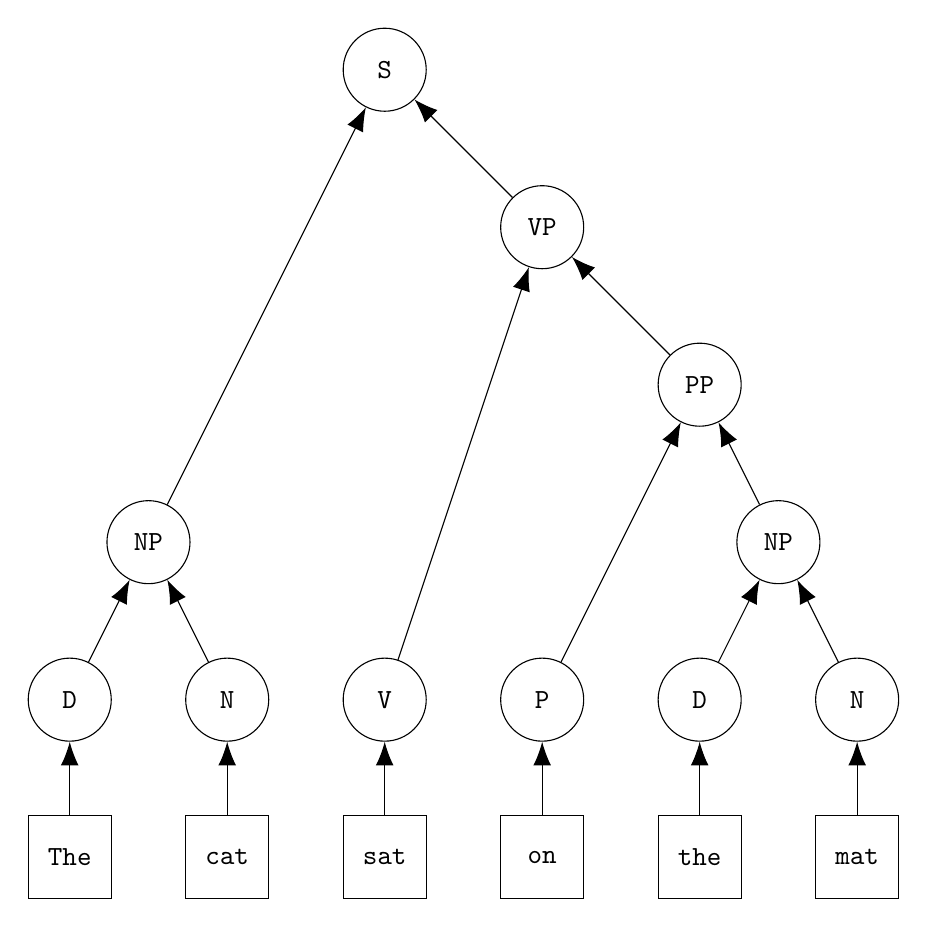
\begin{tikzpicture}[
  scale=1.0,
  cnode/.style={draw,circle,minimum size=3em,inner sep=3pt},
  snode/.style={draw,rectangle,minimum size=3em,inner sep=3pt}
]
  % tokens
  \node[snode] (y1) at (0,0) {$\texttt{The}$};
  \node[snode] (y2) at (2,0) {$\texttt{cat}$};
  \node[snode] (y3) at (4,0) {$\texttt{sat}$};
  \node[snode] (y4) at (6,0) {$\texttt{on}$};
  \node[snode] (y5) at (8,0) {$\texttt{the}$};
  \node[snode] (y6) at (10,0) {$\texttt{mat}$};

  % states
  \node[cnode] (s1) at (0, 2) {$\texttt{D}$};
  \node[cnode] (s2) at (2, 2) {$\texttt{N}$};
  \node[cnode] (s3) at (4, 2) {$\texttt{V}$};
  \node[cnode] (s4) at (6, 2) {$\texttt{P}$};
  \node[cnode] (s5) at (8, 2) {$\texttt{D}$};
  \node[cnode] (s6) at (10, 2) {$\texttt{N}$};

  % token edges
  \draw[-{Latex[length=3mm]}] (y1) edge (s1);
  \draw[-{Latex[length=3mm]}] (y2) edge (s2);
  \draw[-{Latex[length=3mm]}] (y3) edge (s3);
  \draw[-{Latex[length=3mm]}] (y4) edge (s4);
  \draw[-{Latex[length=3mm]}] (y5) edge (s5);
  \draw[-{Latex[length=3mm]}] (y6) edge (s6);

  % hierarchy nodes
  \node[cnode] (s12) at (1, 4) {$\texttt{NP}$};
  \node[cnode] (s56) at (9, 4) {$\texttt{NP}$};
  \node[cnode] (s46) at (8, 6) {$\texttt{PP}$};
  \node[cnode] (s36) at (6, 8) {$\texttt{VP}$};
  \node[cnode] (s16) at (4, 10) {$\texttt{S}$};

  % parsing edges
  \draw[-{Latex[length=3mm]}] (s1) edge (s12);
  \draw[-{Latex[length=3mm]}] (s2) edge (s12);
  \draw[-{Latex[length=3mm]}] (s5) edge (s56);
  \draw[-{Latex[length=3mm]}] (s6) edge (s56);
  \draw[-{Latex[length=3mm]}] (s4) edge (s46);
  \draw[-{Latex[length=3mm]}] (s56) edge (s46);
  \draw[-{Latex[length=3mm]}] (s3) edge (s36);
  \draw[-{Latex[length=3mm]}] (s46) edge (s36);
  \draw[-{Latex[length=3mm]}] (s12) edge (s16);
  \draw[-{Latex[length=3mm]}] (s36) edge (s16);

\end{tikzpicture}
\end{figure}

%%%%%%%%%%%%%%%%%%%%%%%%%%%%%%%%%%%%%%%%%%%%%
% hierarchical derivation with sequential dependencies
\begin{figure}[hbt]
\centering
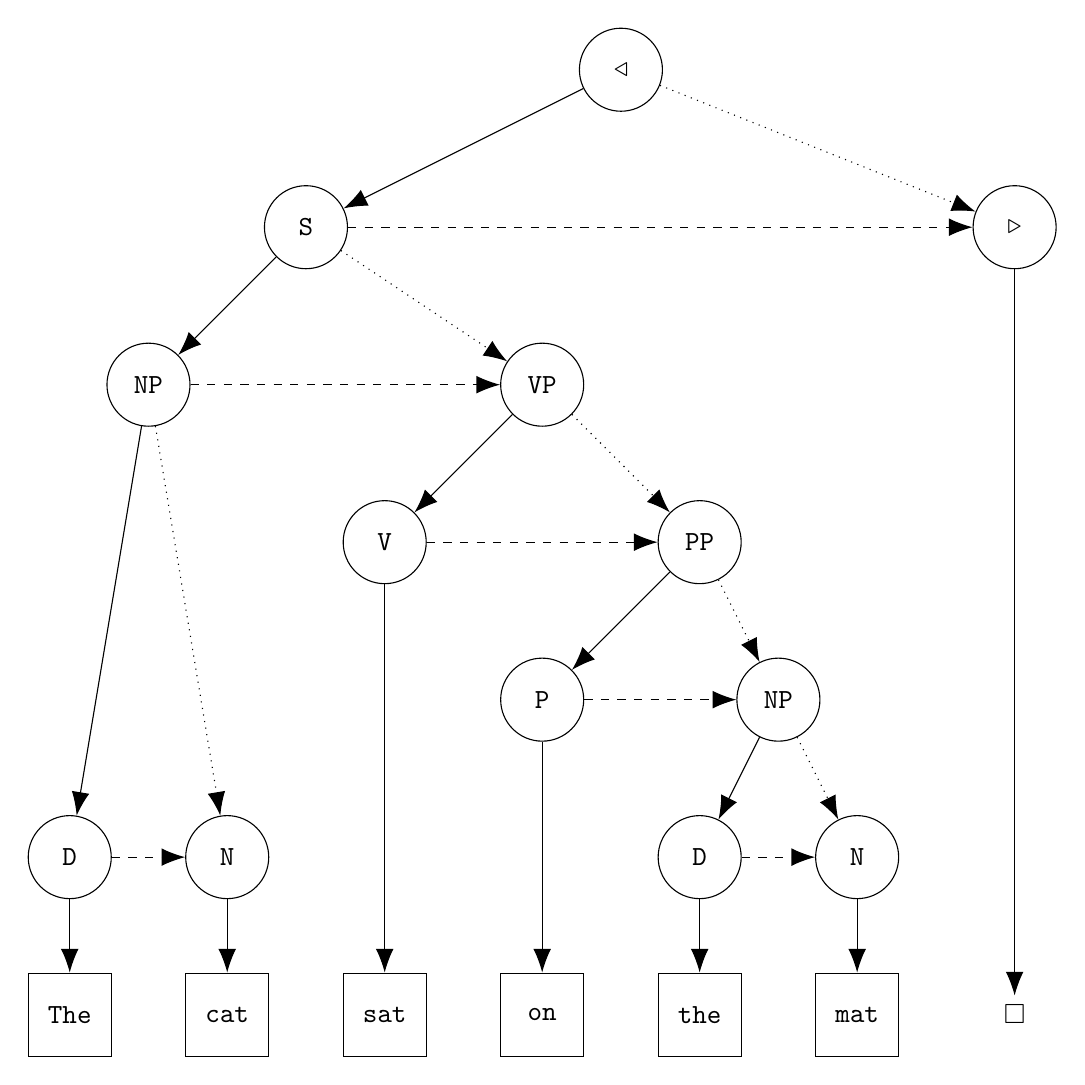
\begin{tikzpicture}[
  scale=1.0,
  cnode/.style={draw,circle,minimum size=3em,inner sep=3pt},
  snode/.style={draw,rectangle,minimum size=3em,inner sep=3pt}
]
  % tokens
  \node[snode] (y1) at (0,0) {$\texttt{The}$};
  \node[snode] (y2) at (2,0) {$\texttt{cat}$};
  \node[snode] (y3) at (4,0) {$\texttt{sat}$};
  \node[snode] (y4) at (6,0) {$\texttt{on}$};
  \node[snode] (y5) at (8,0) {$\texttt{the}$};
  \node[snode] (y6) at (10,0) {$\texttt{mat}$};
  \node (y_end) at (12,0) {$\square$}; % \blacksquare

  % states
  \node[cnode] (s1) at (0, 2) {$\texttt{D}$};
  \node[cnode] (s2) at (2, 2) {$\texttt{N}$};
  \node[cnode] (s3) at (4, 6) {$\texttt{V}$};
  \node[cnode] (s4) at (6, 4) {$\texttt{P}$};
  \node[cnode] (s5) at (8, 2) {$\texttt{D}$};
  \node[cnode] (s6) at (10, 2) {$\texttt{N}$};
  \node[cnode] (s_end) at (12, 10) {$\triangleright$};

  % token edges
  \draw[-{Latex[length=3mm]}] (s1) edge (y1);
  \draw[-{Latex[length=3mm]}] (s2) edge (y2);
  \draw[-{Latex[length=3mm]}] (s3) edge (y3);
  \draw[-{Latex[length=3mm]}] (s4) edge (y4);
  \draw[-{Latex[length=3mm]}] (s5) edge (y5);
  \draw[-{Latex[length=3mm]}] (s6) edge (y6);
  \draw[-{Latex[length=3mm]}] (s_end) edge (y_end);

  % hierarchy nodes
  \node[cnode] (s_start) at (7, 12) {$\triangleleft$};
  \node[cnode] (s16) at (3, 10) {$\texttt{S}$};
  \node[cnode] (s12) at (1, 8) {$\texttt{NP}$};
  \node[cnode] (s56) at (9, 4) {$\texttt{NP}$};
  \node[cnode] (s46) at (8, 6) {$\texttt{PP}$};
  \node[cnode] (s36) at (6, 8) {$\texttt{VP}$};

  % hierarchy edges
  \draw[-{Latex[length=3mm]}] (s_start) edge (s16);
  \draw[-{Latex[length=3mm]},dotted] (s_start) edge (s_end);
  \draw[-{Latex[length=3mm]}] (s12) edge (s1);
  \draw[-{Latex[length=3mm]},dotted] (s12) edge (s2);
  \draw[-{Latex[length=3mm]},dashed] (s12) edge (s36);
  \draw[-{Latex[length=3mm]},dashed] (s1) edge (s2);
  \draw[-{Latex[length=3mm]}] (s56) edge (s5);
  \draw[-{Latex[length=3mm]},dotted] (s56) edge (s6);
  \draw[-{Latex[length=3mm]},dashed] (s5) edge (s6);
  \draw[-{Latex[length=3mm]}] (s46) edge (s4);
  \draw[-{Latex[length=3mm]},dotted] (s46) edge (s56);
  \draw[-{Latex[length=3mm]},dashed] (s4) edge (s56);
  \draw[-{Latex[length=3mm]}] (s36) edge (s3);
  \draw[-{Latex[length=3mm]},dotted] (s36) edge (s46);
  \draw[-{Latex[length=3mm]},dashed] (s3) edge (s46);
  \draw[-{Latex[length=3mm]}] (s16) edge (s12);
  \draw[-{Latex[length=3mm]},dashed] (s16) edge (s_end);
  \draw[-{Latex[length=3mm]},dotted] (s16) edge (s36);

\end{tikzpicture}
\end{figure}


%%%%%%%%%%%%%%%%%%%%%%%%%%%%%%%%%%%%%%%%%%%%%
% Context-sensitive derivation of "The black cat purred.""
\begin{figure}[hbt]
\centering
\begin{tikzpicture}[
  scale=1.5,
  snode/.style={draw,rectangle,minimum size=3em,inner sep=3pt},
  every edge quotes/.style = {auto, font=\footnotesize}
]
  % tokens
  \node[snode] (y1) at (0,0) {$\texttt{The}$};
  \node[snode] (y2) at (2,0) {$\texttt{black}$};
  \node[snode] (y3) at (4,0) {$\texttt{cat}$};
  \node[snode] (y4) at (6,0) {$\texttt{purred}$};

  % leaf states and symbols
  \node (s1) at (0, 2) {$\langle(\texttt{D}$};
  \node (s2) at (2, 2) {$\texttt{J}$};
  \node (s3) at (4, 2) {$\texttt{N})$};
  \node (s4) at (6, 2) {$(\texttt{V}$};
  \node (s4c) at (7, 2) {$)\rangle$};

  % intermediate states
  \node (s13) at (0,4) {$\langle(\texttt{NP}$};
  \node (s13c) at (4,4) {$\oplus$};
  \node (s44) at (6,4) {$\texttt{VP}$};
  \node (s44c) at (7,4) {$)\rangle$};

  % root states
  \node (s14) at (0,6) {$\langle(\texttt{S}$};
  \node (s14c) at (7,6) {$)\rangle$};

  % leaf edges
  \draw[-{Latex[length=3mm]},dotted] (s1) edge["D"] (y1);
  \draw[-{Latex[length=3mm]}] (s1) edge["NP"] (s2);
  \draw[-{Latex[length=3mm]},dotted] (s2) edge["J"] (y2);
  \draw[-{Latex[length=3mm]}] (s2) edge["NP"] (s3);
  \draw[-{Latex[length=3mm]},dotted] (s3) edge["N"] (y3);
  \draw[-{Latex[length=3mm]},dotted] (s4) edge["V"] (y4);

  % intermediate edges
  \draw[-{Latex[length=3mm]}] (s13) edge["NP"] (s1);
  \draw[-{Latex[length=3mm]}] (s3) edge["NP"] (s13c);
  \draw[-{Latex[length=3mm]}] (s13c) edge["S"] (s44);
  \draw[-{Latex[length=3mm]}] (s44) edge["V"] (s4);
  \draw[-{Latex[length=3mm]}] (s4c) edge["V"] (s44c);

  % root edges
  \draw[-{Latex[length=3mm]}] (s14) edge["S"] (s13);
  \draw[-{Latex[length=3mm]}] (s44c) edge["S"] (s14c);

\end{tikzpicture}
\end{figure}

%%%%%%%%%%%%%%%%%%%%%%%%%%%%%%%%%%%%%%%%%%%%%
% Context-free, top-down derivation of "The black cat purred.""
\begin{figure}[hbt]
\centering
\begin{tikzpicture}[
  scale=1.5,
  snode/.style={draw,rectangle,minimum size=3em,inner sep=3pt},
  every edge quotes/.style = {auto, font=\footnotesize}
]
  % tokens
  \node[snode] (y1) at (0,0) {$\texttt{The}$};
  \node[snode] (y2) at (2,0) {$\texttt{black}$};
  \node[snode] (y3) at (4,0) {$\texttt{cat}$};
  \node[snode] (y4) at (6,0) {$\texttt{purred}$};

  % leaf states and symbols
  \node (s1) at (0, 2) {$\langle(\texttt{D}$};
  \node (s2) at (2, 2) {$\texttt{J}$};
  \node (s3) at (4, 2) {$\texttt{N})$};
  \node (s4) at (6, 2) {$(\texttt{V}$};
  \node (s4c) at (7, 2) {$)\rangle$};

  % intermediate states
  \node (s13) at (0,4) {$\langle(\texttt{NP}$};
  \node (s44) at (6,4) {$\texttt{VP}$};
  \node (s44c) at (7,4) {$)\rangle$};

  % root states
  \node (s14) at (0,6) {$\langle(\texttt{S}$};
  \node (s14c) at (7,6) {$)\rangle$};

  % leaf edges
  \draw[-{Latex[length=3mm]},dotted] (s1) edge (y1);
  \draw[-{Latex[length=3mm]}] (s1) edge (s2);
  \draw[-{Latex[length=3mm]},dotted] (s2) edge (y2);
  \draw[-{Latex[length=3mm]}] (s2) edge (s3);
  \draw[-{Latex[length=3mm]},dotted] (s3) edge (y3);
  \draw[-{Latex[length=3mm]},dotted] (s4) edge (y4);

  % intermediate edges
  \draw[-{Latex[length=3mm]}] (s13) edge (s1);
  \draw[-{Latex[length=3mm]}] (s3) edge (s44);
  \draw[-{Latex[length=3mm]}] (s44) edge (s4);
  \draw[-{Latex[length=3mm]}] (s4c) edge (s44c);

  % root edges
  \draw[-{Latex[length=3mm]}] (s14) edge (s13);
  \draw[-{Latex[length=3mm]}] (s44c) edge (s14c);

\end{tikzpicture}
\end{figure}

%%%%%%%%%%%%%%%%%%%%%%%%%%%%%%%%%%%%%%%%%%%%%
% Context-free, bottom-up derivation of "The black cat purred.""
\begin{figure}[hbt]
\centering
\begin{tikzpicture}[
  scale=1.5,
  snode/.style={draw,rectangle,minimum size=3em,inner sep=3pt},
  every edge quotes/.style = {auto, font=\footnotesize}
]
  % tokens
  \node[snode] (y1) at (0,0) {$\texttt{The}$};
  \node[snode] (y2) at (2,0) {$\texttt{black}$};
  \node[snode] (y3) at (4,0) {$\texttt{cat}$};
  \node[snode] (y4) at (6,0) {$\texttt{purred}$};

  % leaf states and symbols
  \node (s1) at (0, 2) {$\langle(\texttt{D}$};
  \node (s2) at (2, 2) {$\texttt{J}$};
  \node (s3) at (4, 2) {$\texttt{N})$};
  \node (s4) at (6, 2) {$(\texttt{V})\rangle$};

  % intermediate states
  \node (s13) at (4,4) {$\langle(\texttt{NP}$};
  \node (s44) at (6,4) {$\texttt{VP})\rangle$};

  % root states
  \node (s14) at (6,6) {$\langle(\texttt{S})\rangle$};

  % leaf edges
  \draw[-{Latex[length=3mm]},dotted] (s1) edge (y1);
  \draw[-{Latex[length=3mm]}] (s1) edge (s2);
  \draw[-{Latex[length=3mm]},dotted] (s2) edge (y2);
  \draw[-{Latex[length=3mm]}] (s2) edge (s3);
  \draw[-{Latex[length=3mm]},dotted] (s3) edge (y3);
  \draw[-{Latex[length=3mm]},dotted] (s4) edge (y4);

  % intermediate edges
  \draw[-{Latex[length=3mm]}] (s3) edge (s13);
  \draw[-{Latex[length=3mm]}] (s13) edge (s4);
  \draw[-{Latex[length=3mm]}] (s4) edge (s44);

  % root edges
  \draw[-{Latex[length=3mm]}] (s44) edge (s14);

\end{tikzpicture}
\end{figure}

%%%%%%%%%%%%%%%%%%%%%%%%%%%%%%%%%%%%%%%%%%%%%
% Top-down hierarchy of "The black cat purred.""
\begin{figure}[hbt]
\centering
\begin{tikzpicture}[
  scale=1.5,
  snode/.style={draw,rectangle,minimum size=3em,inner sep=3pt},
  every edge quotes/.style = {auto, font=\footnotesize}
]
  % tokens
  \node[snode] (y1) at (0,0) {$\texttt{The}$};
  \node[snode] (y2) at (2,0) {$\texttt{black}$};
  \node[snode] (y3) at (4,0) {$\texttt{cat}$};
  \node[snode] (y4) at (6,0) {$\texttt{purred}$};

  % leaf states and symbols
  \node (s1) at (0, 2) {$(\texttt{D}$};
  \node (s2) at (2, 2) {$\texttt{J}$};
  \node (s3) at (4, 2) {$\texttt{N})$};
  \node (s4) at (6, 2) {$(\texttt{V})$};

  % intermediate states
  \node (s13) at (4,4) {$(\texttt{NP}$};
  \node (s44) at (6,4) {$\texttt{VP})$};

  % root states
  \node (s14) at (6,6) {$\langle\texttt{S}\rangle$};

  % leaf edges
  \draw[-{Latex[length=3mm]},dotted] (s1) edge (y1);
  \draw[-{Latex[length=3mm]}] (s1) edge (s2);
  \draw[-{Latex[length=3mm]},dotted] (s2) edge (y2);
  \draw[-{Latex[length=3mm]}] (s2) edge (s3);
  \draw[-{Latex[length=3mm]},dotted] (s3) edge (y3);
  \draw[-{Latex[length=3mm]},dotted] (s4) edge (y4);

  % intermediate edges
  \draw[-{Latex[length=3mm]}] (s13) edge (s1);
  \draw[-{Latex[length=3mm]},dashed] (s13) edge (s2);
  \draw[-{Latex[length=3mm]},dashed] (s13) edge (s3);
  \draw[-{Latex[length=3mm]}] (s44) edge (s4);

  % root edges
  \draw[-{Latex[length=3mm]}] (s14) edge (s13);
  \draw[-{Latex[length=3mm]}] (s14) edge (s44);

\end{tikzpicture}
\end{figure}

\end{document}
